\documentclass[spanish,12pt]{elsarticle}
\usepackage{graphicx}
\usepackage{amssymb}
\usepackage{amsmath}
\usepackage{siunitx}
\usepackage{lineno}
\usepackage{babel}
\usepackage{listings}
\usepackage{xcolor}
\newcommand{\blank}[1]{\hspace*{#1}}
\definecolor{codegreen}{rgb}{0,0.6,0}
\definecolor{codegray}{rgb}{0.5,0.5,0.5}
\definecolor{codepurple}{rgb}{0.58,0,0.82}
\definecolor{backcolour}{rgb}{0.95,0.95,0.92}
\lstdefinestyle{mystyle}{
    backgroundcolor=\color{backcolour},   
    commentstyle=\color{codegreen},
    keywordstyle=\color{magenta},
    numberstyle=\tiny\color{codegray},
    stringstyle=\color{codepurple},
    basicstyle=\ttfamily\footnotesize,
    breakatwhitespace=false,         
    breaklines=true,                 
    captionpos=b,                    
    keepspaces=true,                 
    numbers=left,                    
    numbersep=5pt,                  
    showspaces=false,                
    showstringspaces=false,
    showtabs=false,                  
    tabsize=2
}
\lstset{style=mystyle}
\makeatletter
\def\ps@pprintTitle{%
  \let\@oddhead\@empty
  \let\@evenhead\@empty
  \let\@oddfoot\@empty
  \let\@evenfoot\@oddfoot
}
\makeatother

\abstracttitle{Resumen}

\begin{document}

\begin{frontmatter}
\title{Problema K-minimum spanning tree}
\author{Roberto Juan Cayro Cuadros, Gabriel Alexander Valdivia Medina,
Giulia Alexa Naval Fernández, Rodrigo Alonso Torres Sotomayor}
\begin{abstract}
    El presente trabajo presenta una breve investigación del problema \textit{k-minimun spanning tree}, explicando su funcionamiento, demostrando que pertenece al conjunto de los problemas NP-completos, y dando opciones de algoritmos para su resolución.\\
\end{abstract}
\address{Universidad Católica San Pablo}

\end{frontmatter}

%%
%% Start line numbering here if you want
%%

%% main text
\section {Conocimientos previos}
\subsection{Problemas de la clase P}
Los problemas de la clase P (Polynomial time) son todos aquellos que se pueden resolver en tiempo polinomial. Es decir, pueden ser resueltos polinomialmente en el mundo real. Entre los problemas más conocidos se encuentran la búsqueda del elemento mínimo, la ordenación de un conjunto de elementos, encontrar un árbol mínimo de expansión, etc.


\subsection{Problemas de la clase NP}
Los problemas de la clase NP (Non-deterministic polynomial time) son aquellos que pueden ser resueltos en tiempo polinomial usando una máquina o un algoritmo \textbf{no determinístico}. En la mayoría de casos, estos algoritmos no se pueden representar adecuadamente en la vida real por su carácter no determinístico. Sin embargo, los problemas NP se pueden verificar con facilidad, siendo verificables en tiempo polinomial.
Algunos ejemplos conocidos pueden ser el camino Hamiltoniano, la coloración de grafos, entre otros.
\clearpage


\subsection{Relación entre NP y P}
Uno de los problemas más famosos de la computación es el determinar si $P = NP$. Se sabe que $P \subset NP$, ya que ambos pueden comprobarse en tiempo polinomilal. Sin embargo, para demostrar que $P=NP$ se tendría que demostrar que existe una solución polinomial para los NP, cosa que no ha sido demostrada hasta la fecha y que se cree que nunca lo será.


\subsection{Problemas de la clase NP-hard}
A pesar del nombre, no todos los problemas NP-hard pertenecen a NP. La principal característica de estos problemas es que son por lo menos tan difíciles como el problema NP más difícil. Además, todo problema que pertenece a la clase NP se puede transformar o reducir a un problema NP-hard. Por otro lado, estos problemas son mucho más difíciles de verificar que los NP. Algunos ejemplos conocidos son el problema de detención (halting problem) y hallar un camino \textbf{no Hamiltoniano}.


\subsection{Problemas de clase NP-completo}
Los NP- completo son un tipo especial de problema, todos los problemas NP-completo pertenecen a su vez tanto a los NP como a los NP-hard. Su peculiaridad principal es que todo problema NP-completo puede reducirse a cualquier otro problema NP-completo en \textbf{tiempo polinomial}. Por lo tanto, si se pudiera encontrar una solución polinomial para cualquier problema NP-completo, entonces se podrían encontrar también soluciones polinomiales para todos los problemas del conjunto. Algunos problemas conocidos son el ciclo Hamiltoniano, SAT, entre otros. La manera más fácil de demostrar que un problema pertenece a los NP-completos es primero demostrar que pertenece a NP, con un algoritmo no determinístico en tiempo polinomial. Y luego, demostrar que un problema NP-completo ya conocido puede transformarse para ser resuelto por el algoritmo de este problema.
\clearpage



\section{Introducción al problema k-MST}
Según múltiples fuentes\cite{3}\cite{5}, el k-MST o k-minnimum spanning tree problem, árbol de expansión de péso mínimo k en español es un problema computacional que pide un árbol de mínimo costo con exactamente $k$ vértices que forme un subgrafo del grafo original.
\begin{figure}[h]
    \centering
    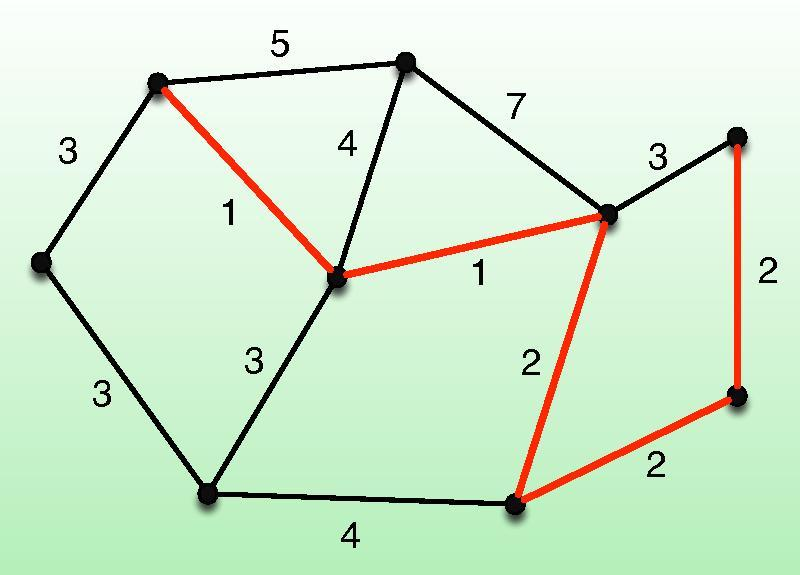
\includegraphics[scale=0.45]{images/6-mst.jpg}
    \caption{6-MST del grafo G. Fuente: Wikipedia Commons}
    \label{fig:my_label}
\end{figure}
%---------------------------------------------------------%


\section{Demostración NP-completo}
\paragraph{\textnormal{No es posible suponer la naturaleza del problema, y establecer que es NP-hard o NP-completo, sin la evidencia correspondiente, para probrarlo este debe pertenecer a NP, ademas que un problema NP-completo pueda reducirse al mismo}}
\subsection{Demostrar que k-MST $\in$ NP}
Para demostrar que un problema pertenece a la clase NP, se debe crear un algoritmo no deterministico que resuelva el problema en tiempo polinomial:\\\\
\textit{\underline{k-MST (G,k)} }
\begin{enumerate}
    \item  \textnormal{t $\leftarrow$ 0}
    \item  \textnormal{\textbf{while} t $<$ k}
    \item \textnormal{\blank{1cm}\textbf{do} u $\leftarrow${ESCOGER(G)}}
    \item  \textnormal{\blank{2cm}\textbf{if} u \textbf{is not in} x}
    \item \textnormal{\blank{3cm}\textbf{do} x . add(u)}
     \item \textnormal{\blank{3cm} t++}\\
\end{enumerate}
X será el árbol a construirse,junto con el bucle while y una variable t confirmaremos la adición de  exactamente k vértices, escogeremos algún \textit{u} de \textit{G}, si \textit{u} ya esta dentro de \textit{x} el valor de t no cambie por lo tanto se repite hasta tomar otro vértice.

\subsection{Transformación NP-completo $\alpha$  k-MST}
El segundo paso para demostrar que un problema pertenece a los NP-completos, es transformar un problema NP-completo conocido para que pueda ser resuelto por el algoritmo del k-MST. Una transformación sencilla es la que se puede hacer dese el problema de Steiner.
\subsubsection{Steiner problem}
Según el artículo de Shivam Gupta\cite{2}, el Steiner problem es un problema NP-completo de los 21 problemas de Karp, usado en problemas de optimización y mayormente enfocado en estructuras de grafos aunque tambien visto en aplicaciones de modelación de redes con más de 2 terminales. El problema consiste en que, dado un grafo no-dirigido de aristas con peso, generar un arbol dado un
\textit{Sub-set} de vertices los cuales formarán este arbol. Además, pueden añadirse nuevos vertices del grafo al \textit{sub-set} para lograr las conexiones entre estos, llamados \textit{Steiner-vertices}.\\

La decisión asociada al problema será averiguar si existe un árbol que una todos los vértices de un \textit{sub-set} $R$, usando máximo $M$ aristas. Los vertices deberán ser exactamente los dados en el Sub-set. Esta decisión es conocida por ser del grupo de los NP-completos.
La principal diferencia con el k-MST es que aquí recibimos un conjunto específico de vectores para conformar nuestro árbol, pudiendo usar vértices fuera de la relación para conectarlos. El k-MST no recibe esta relación, sólo el número de vértices exactos que necesita.\\ 


\subsection{Entradas y salidas}


\subsubsection*{\underline{Steiner-tree}}

\begin{center}
\begin{tabular}{ |l| }
\hline
Steiner-problem \\ \hline
\textit{Entrada: }\\
\blank{1cm} *Grafo no-dirigido G con aristas de peso. \\
\blank{1cm} *Sub-set de vertices R. \\
\blank{1cm} *Número M. \\
\\\hline
\textit{Salida: } \\
\blank{1cm} *Arbol de menor peso con los vertices de S \\
\blank{1cm}y los Steiner-vertices si fueran necesarios.\\
\\\hline
\end{tabular}
\end{center}

\subsubsection*{\underline{k-MST}}
\begin{center}
\begin{tabular}{ |l| }
\hline
k-MST \\ \hline
\textit{Entrada: }\\
\blank{1cm} *Grafo no-dirigido G con aristas de peso. \\
\blank{1cm} *Número k de vértices. \\

\\\hline
\textit{Salida: } \\
\blank{1cm} *Arbol de menor peso con k-vertices y k-1, \\
\blank{1cm}aristas.\\

\\\hline
\end{tabular}
\end{center}


\subsubsection{Transformación}
\textnormal{Una primera aproximación será que dada la entrada G para Steiner, se puede tomar el mismo grafo para k-MST, puesto que tiene las aristas pesadas y un número determinado de vertices. De esta forma aseguramos la transformación y no afectara la salida porque siempre busaremos el arbol de menor peso , se usará el tamaño del sub-set de vertices siendo este igual a k.}\\\\
\textnormal{Pero no podemos asegurar que esta transformación pudiera también resolver al Steiner tree, siendo esta una de las propiedades en una transformación polinómica. Como tenemos de entrada un G, y k, podriamos calcular todas las permutaciones de G en k. Y necesariamente una de ellas corresponderia a la solución para Steiner:}\\\\
\textit{
\[
\textnormal{Total~de~permutaciones (Tn)}= \binom{n}{k} = \frac{n!}{k!(n - k)! }.
\]
}

\[
S \subseteq Tn.
\]
Sin embargo, calcular todas las permutaciones de una cantidad $n$ de elementos es un proceso con una complejidad $O(!n)$, que no entra dentro de complejidad polinomial, además que esta reducción planteada no resolverá el problema de k-MST, ya que este necesitaría solo 1 árbol de menor peso. Es necesario entonces otro tratamiento para que el k-MST opere con los vértices que el algoritmo Steiner pide. Siguiendo la transformación de R. Ravi \cite{4}, otra idea es añadir un árbol con aristas de peso 0 en cada vértice que pertenezca a R, y transformar $k$ como $k = |R|(X+1)$, siendo X la cantidad de vértices que tendrán cada uno de estos árboles, denotado como $X = |V(G)|-|R|$ De esta forma, el k-MST utilizará los vértices de $R$ sí o sí como parte de su solución.
\\\\ 
\begin{figure}[h]
    \centering
    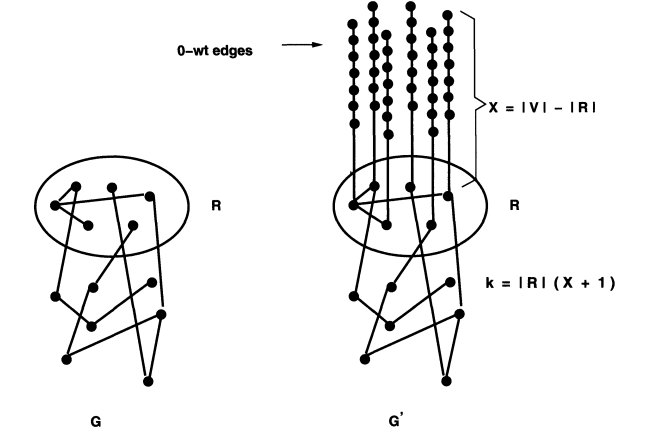
\includegraphics[scale=0.65]{images/graph_explicacion.png}
    \caption{Transformación de la entrada de Steiner a entrda de k-MST. Fuente: www.contrib.andrew.cmu.edu }
    \label{fig:my_label}
\end{figure}
\\\\
En este nuevo grafo $G'$, las aristas que unen los nuevos vértices de X tendrán un peso de 0, las aristas correspondientes a las aristas originales de G tendrán un peso de 1, y el resto de pares del grafo tendrán un peso de $\infty$. De este modo, el algoritmo del k-MST encontrará el árbol de menor peso con el parámetro k en $G'$, y verificará si es de igual o menor peso que M, satisfaciendo el requisito de las M aristas debido a que estas tendrán peso 1.\\\\
Por otra parte cumpliremos la propiedad de la transformación polinomial, en donde redujimos el problema de Steiner a k-MST, por ello la solución a k-MST mediante otra transformación polinómica podra ser la solución a Steiner-tree, gracias al valor de la transformación de k= a (X+1)|R|, puesto que las aristas de los árboles agregados son de peso 0, estos serán agregados a la solución y por el k se confirma que en la solución de k-MST estarán los vértices de R.


 
\section{Algoritmo de fuerza bruta}
Para el algoritmo de fuerza bruta, es suficiente una modificación al algoritmo Prim convencional, limitando su avance a k nodos y haciendo que se repita con cada nodo del grafo G como origen. Finalmente, decidir qué arbol de todos los obtenidos ha sido el más corto.

\subsection{Algoritmo de prim.}
Es un \textit{algoritmo greedy}, que dado un grafo \textit{G}  encuentra el MST(Minimun-spanning-tree) de menor peso posible, usando todos los vértices de G y donde el peso total es el mínimo. El algoritmo funciona un vértice a la vez buscando la conexión al siguiente vértice de menor peso de la forma:\\
\begin{enumerate}
    \item  Iniciar el árbol con un vértice cualquiera del grafo
    \item  Construir el árbol, vértice por vértice usando aquellos vértices que ya no estén agregados
    \item repetir el paso 2 hasta que todos los vértices estén en el árbol

\end{enumerate}

\begin{figure}[h]
    \centering
    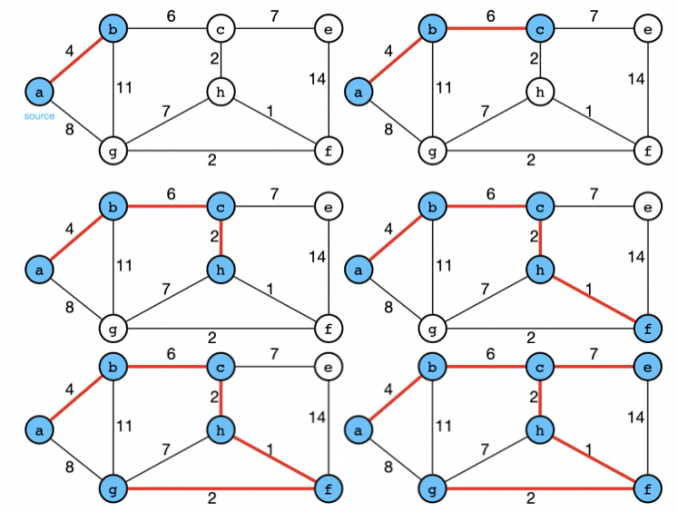
\includegraphics[scale=0.5]{images/prm.png}
    \caption{Funcionamiento de prim. Fuente: https://laptrinhx.com/minimum-spanning-tree-prim-4207877151/ }
    \label{fig:my_label}
\end{figure}
\clearpage


\subsection{Implementación}
\lstinputlisting[language=C++]{codes/BruteForce.cpp}


\subsection{Resultado}
\subsubsection{Entrada}
\begin{figure}[h]
    \centering
    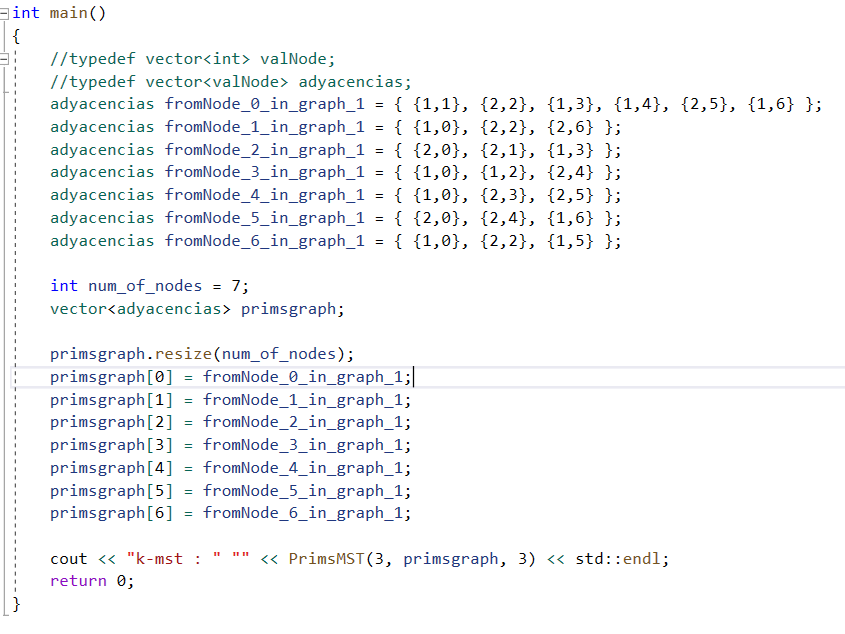
\includegraphics[scale=0.45]{images/FB-entrada.png}
    \caption{Entrada del algoritmo de fuerza bruta. Obtención propia.}
    \label{fig:my_label}
\end{figure}
\subsubsection{Salida}
\begin{figure}[h]
    \centering
    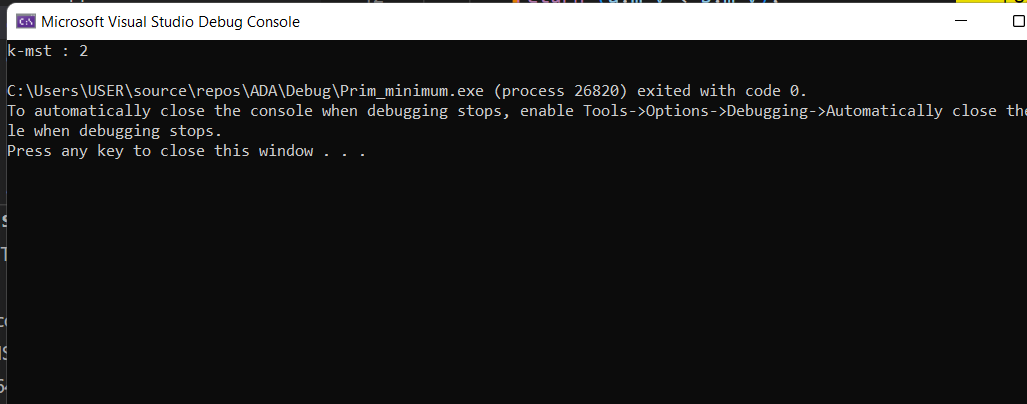
\includegraphics[scale=0.4]{images/FB-salida.png}
    \caption{Salida del algoritmo de fuerza bruta. Obtención propia.}
    \label{fig:my_label}
\end{figure}
\clearpage


\section{Algoritmo aproximado}
\subsection{Idea}
Según el artículo de Subham Datta\cite{1}, \textit{Branch and Bound} es un algoritmo que optimiza otros algoritmos estableciendo limitaciones en el conjunto de respuestas posible. Es usado ampliamente en problemas NP-completos para hallar con facilidad computacional un resultado aproximado. Normalmente los \textit{Upper Bounds} o límites superiores son condiciones que limitan el avance de la cantidad de respuestas, depende de la lógica del problema a tratar pero, en general, se toma un punto específico dentro del área de búsqueda de respuestas.\\\\
En caso del k-MST, se hacen varios tratamientos para que no tenga que buscar exhaustivamente la respuesta desde todos los nodos como origen. Primero se establecen nodos de partida que estén relacionados con aristas de peso muy bajo, luego se elige un valor específico que interrumpa la búsqueda al ser superado. Este es el límite superior. También se hace caso de una enumeración diferente, donde a los nodos se les da un valor precomputarizado de aristas / peso y con ese valor poder decidir qué valores añadir al grafo actual y cuáles no.


\subsection{Implementación}
\lstinputlisting[language=C++]{codes/KMST.cpp}

\clearpage
\section{Aplicaciones}
\subsection{Network Design}
Una de sus aplicaciones más conocidas respecto a problemas de conexión, por ejemplo una compañia de celular, que tiene distintos precios por diferentes pares de ciudades, el problema esta en construir la red de menor costo posible dado estas ciudades. O bien para una agencia de viajes, y se busca determinar el alcance y costo de la aerolínea.

\begin{figure}[h]
    \centering
    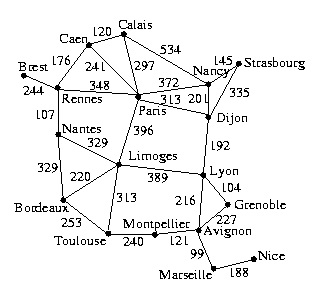
\includegraphics[scale=1.00]{images/ciudades.jpg}
    \caption{Grafo de ciudades. Fuente: https://people.cs.georgetown.edu/~maloof/cosc270.f17/p2.html }
    \label{fig:my_label}
\end{figure}



\bibliographystyle{model1-num-names}
\appendix
\bibliography{sample.bib}
\clearpage
\begin{thebibliography}{00}
\bibitem{1}Datta, S. (10 de Octubre de 2020). baeldung.com. Obtenido de https://www.baeldung.com/cs/branch-and-bound
\bibitem{2} Gupta, S. (Junio de 2022). geeksforgeeks. Obtenido de https://www.geeksforgeeks.org/steiner-tree/
\bibitem{3}Matt Elder, S. C. (2007). CS880: Approximation Algorithms. Obtenido de https://pages.cs.wisc.edu/~shuchi/courses/880-S07/scribe-notes/lecture26-2.pdf
\bibitem{4}R. Ravi, R. S. (12 de Julio de 2006). Spanning Trees—Short or Small. Obtenido de SIAM (Society for Industrial and Applied Mathematics: https://epubs.siam.org/doi/pdf/10.1137/S0895480194266331
\bibitem{5} Wikipedia. (Junio de 2022). Wikipedia. Obtenido de https://en.wikipedia.org/wiki/K-minimum$_$spanning$_$tree
\end{thebibliography}
%https://en.wikipedia.org/wiki/K-minimum_spanning_tree
%https://www.geeksforgeeks.org/steiner-tree/
%https://pages.cs.wisc.edu/~shuchi/courses/880-S07/scribe-notes/lecture26-2.pdf
%https://www.contrib.andrew.cmu.edu/~ravi/sidma96.pdf
%https://www.baeldung.com/cs/branch-and-bound
\end{document}